%Project       : Resources, HelperFile
%Description: helper file to write LaTeX documents   
%Basics:	
%This version: 10/24/2014
%This .tex file:   Jorge Luis Garcia
%This project : CEHD

%Style
\documentclass[11pt]{article}
\usepackage[top=1in, bottom=1in, left=1in, right=1in]{geometry}
\parindent 22pt

%Packages
\usepackage{adjustbox}
\usepackage{amsmath}
\usepackage{amsfonts}
\usepackage{amssymb}
\usepackage{bm}
\usepackage[table]{xcolor}
\usepackage{tabu}
\usepackage{makecell}
\usepackage{longtable}
\usepackage{multirow}
\usepackage[normalem]{ulem}
\usepackage{etoolbox}
\usepackage{graphicx}
\usepackage{tabularx}
\usepackage{ragged2e} 
\usepackage{booktabs}
\usepackage{caption}
\usepackage[none]{hyphenat}
\usepackage{fixltx2e}
\usepackage{threeparttablex}
\usepackage[capposition=top]{floatrow}
\usepackage{subcaption}
\usepackage{pdfpages}
\usepackage{pdflscape}
\usepackage{natbib}
\definecolor{maroon}{HTML}{990012}
\usepackage[colorlinks=true,linkcolor=maroon,citecolor=maroon]{hyperref}
%\doublespacing

%Functions
\DeclareMathOperator{\cov}{Cov}
\DeclareMathOperator{\var}{Var}
\DeclareMathOperator{\plim}{plim}

%Math Environments
\newtheorem{theorem}{Theorem}
\newtheorem{assumption}[theorem]{Assumption}
\newtheorem{condition}[theorem]{Condition}
\newtheorem{example}[theorem]{Example}
\newtheorem{exercise}[theorem]{Exercise}
\newtheorem{remark}[theorem]{Remark}
\newtheorem{claim}[theorem]{Claim}
\newtheorem{lemma}[theorem]{Lemma}
\newtheorem{definition}[theorem]{Definition}
\newtheorem{hypothesis}[theorem]{Hypothesis}
\newtheorem{property}[theorem]{Property}
\newenvironment{proof}[1][Proof]{\noindent\textbf{#1.} }{\ \rule{0.5em}{0.5em}}

%Independent
\newcommand\independent{\protect\mathpalette{\protect\independenT}{\perp}}
\def\independenT#1#2{\mathrel{\rlap{$#1#2$}\mkern2mu{#1#2}}}
%Overbar
\newcommand{\overbar}[1]{\mkern 1.5mu\overline{\mkern-1.5mu#1\mkern-1.5mu}\mkern 1.5mu}
%Identical in distribution
\newcommand{\equald}{\ensuremath{\overset{d}{=}}}
%Special doubled cell in a table
\newcommand{\specialcell}[2][c]{%
  \begin{tabular}[#1]{@{}c@{}}#2\end{tabular}}

\renewcommand{\rothead}[2][60]{\makebox[9mm][c]{\rotatebox{#1}{\makecell[c]{#2}}}}
\newcommand{\mr}{\multirow}
\newcommand{\mc}{\multicolumn}

\begin{document}

\title{Human Capital 34300 by Professor Gary S. Becker}
\author{}
\date{This draft \today}
\maketitle


\noindent The basis of these notes is the class Gary Becker's Econ 344, Human Capital. Thus, they focus on education in an altruistic model, trade-off between human and physical capital investments, intergenerational income mobility, investments in health, etc. In his work, Becker points out that human capital is special because (i) it has an inextricable link to the human being; (ii) it is durable, like physical capital. The reason why Human Capital is very important in the modern study of economics is because it is a fundamental component of productivity. Importantly, Human Capital is also the most natural link between parents and child. Put differently, Human Capital forms through an investment process parents carry on during their offspring's childhood.\\
\indent There are properties and empirical facts making the study of human capital challenging and interesting. Firstly, almost all forms of human capital are deeply complementary. Empirically, there is a positive correlation between education, health, training, good diet, adequate use of contraception,  marriage stability, adaptation to technology, and even subjective measures of happiness --which economists commonly call into question due to measurement complications. An interesting fact appearing to contradict these empirical regularity is that more educated women marry less. Secondly, the differences between physical and human capital are such that both need, at least for an initial understanding, an exclusive and distinctive field of study. Some of the main differences of human capital with respect to physical capital are the following: (i) human capital cannot be bought because slavery is forbidden; (ii) there is not a market for human capital; (iii) it is almost impossible to use human capital as a collateral. Thirdly, since human capital builds on itself, i.e. human capital is intensive in human capital, children from parents with greater human capital have an advantage which drives social (in) mobility. Fourthly, the benefits of going school began to increase a lot in the 1980s while tuition went up.\\  
\indent To start off and settle down ideas to understand these and other facts we follow Becker's rationale and start by covering the basic one child and one parent model, in which parents and children overlap for a single period.

\section{Unisex Adult Model} \label{sec:unisex}

\noindent This model has the following basic assumptions: (i) there is a representative family with one adult and one child; (ii) there are two periods, childhood and adulthood; (iii) the child and the parent overlap for one period. We denote as $t$ the period in which child and parent overlap. The parent makes a decision in this period. In $t+1$ he dies and his son becomes the adult.\\
\indent The parent decides how to allocate his resources, parental exogenous income, into consumption or children goods --or investment in children. His budget constraint is the following: 

\begin{equation}
\underbrace{C_{p}}_{\text{parental consumption}} + \underbrace{I_{c}}_{\text{investment in children}} = \underbrace{W_{p}}_{\text{parental income}}.
\end{equation}

\indent The child has no way to repay her parent for the investment he makes on her in $t$. Thus, the assumption making the model interesting is that the parent is altruistic, i.e. $I_{C}^* \neq 0$. $a$ is the altruism parameter in the parental utility function

\begin{equation}
U_{p} (W_{p}) = U(C_{p}) + a V (W_{c}) \label{eq:parentutility}
\end{equation}

\noindent where $W_{c}$ is child's income \textit{during adulthood}. A parent is altruistic iff $a > 0$. We assume  \eqref{eq:parentutility} is weakly concave and satisfies standard Inada conditions. Moreover, we assume the human capital production function is strictly concave in parental investment --at least in the region of focus that interests us. Let $H_{c} \equiv f(I_{c})$ denote child's human capital. Hence, $\frac{d H_{c}}{ d I_{c}} > 0, \frac{d^2 H_{c}}{ d I_{c}^2} < 0$. Graphically,

\begin{center}
\begin{figure}[H] 
\caption{Human Capital Production Function: Region of Interest}
\centering
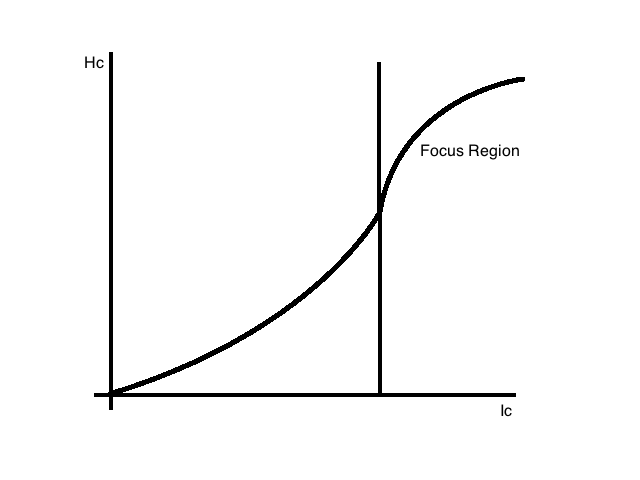
\includegraphics[width=4in, height=3in]{Plots/FocusRegion.png}
\end{figure}
\end{center}

\indent An intuitive way to think of diminishing marginal returns on investment is the following. Let $B$ denote the innate ability of the child, something like the brain. If in our period of study the brain is fixed at a level $\bar{B}$, then it is easy to understand that strict concavity in $I_{c}$. Now, let us close the model by stating some additional assumptions. Let $r$ be the rental rate of human capital. This is, each unit of human capital pays off $r$. Thus, $W_{c} = r H_{c}$. This rate is (i) constant across households; (ii) taken by parents as part of the market environment. Thus, the only reason why earnings differ, at least at this stage of the analysis, is because of human capital --which investment in children, $I_{c}$, constructs.\\

\indent The \textit{economic problem} is the following
\begin{equation}
\max_{I_{c}, C_{p}} \{ U_{p} (W_{p}) = U(C_{p}) + a V(W_{c}) \}
\end{equation}  

\noindent s.t.

\begin{equation}
C_{p} + I_{c} = W_{p}. \label{eq:constraint}
\end{equation}

\begin{center}
\begin{figure}[H] 
\caption{Graphical Representation of the Solution to the Unisex Adult Model}
\centering
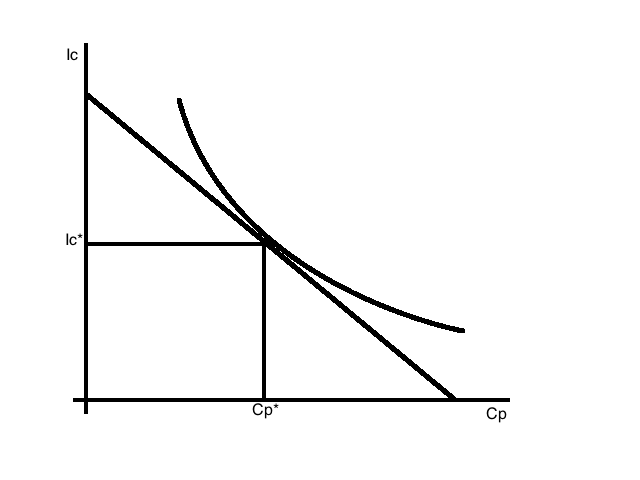
\includegraphics[width=4in, height=3in]{Plots/EconProb.png}
\end{figure}
\end{center}


\indent The condition pinning down equilibrium is 

\begin{equation}
U'(C_{p}) \geq a \frac{d V(W_{c})}{d I_{c}}. \label{eq:mrs}
\end{equation}

\noindent If the parent is altruistic the only reason for $I_{c}^* = 0$ is if his income is very low. Now note that $W_{c} = r H_{c}$ and $\frac{d V(W_{c})}{d I_{c}} = \frac{d V(W_{c})}{d W_{c}} \frac{d W_{c}}{d H_{c}} \frac{d H_{c}}{d I_{c}}$. Moreover, $\frac{d W_{c}}{d H_{c}} = R$, $\frac{d H_{c}}{d I_{c}} \equiv f_{y}$. Hence, we think of $r f_{y} \equiv R_{y}$ as the marginal rate of return of investment in the child, $I_{c}$. Thus we can rewrite \eqref{eq:mrs} as

\begin{equation}
U'(C_{p}) = a V'(\cdot) R_{y}
\end{equation}

\noindent \ldots the marginal utility from consumption has to be equal to the marginal investment of investment in the child, in equilibrium. Now, \eqref{eq:constraint} and \eqref{eq:mrs} are two equations for the two choice variables we want to solve for in this model. Thus, they characterize the equilibrium.\\
\indent Let

\begin{eqnarray}
a r f_i V'_{c} - U'(C_p) = 0 &\Leftrightarrow& g_1 (y_c, C_p; a, r, W_p) = 0 \label{eq:g1} \\
C_p + y_c - W_p = 0 &\Leftrightarrow& g_2 (y_c, C_p; a, r, W_p) = 0.  \label{eq:g2} 
\end{eqnarray}

\noindent By the implicit function theorem,

\begin{align*}
\begin{bmatrix}
    \ \ \frac{dC_p}{dW_p}\ \ \\
    \ \ \frac{dy_c}{dW_p}\ \
\end{bmatrix} &= - \begin{bmatrix}
                    \ \ \frac{dg_1}{dc_p} \quad &\frac{dg_1}{dy_c}\ \ \\
                    \ \ \frac{dg_2}{dc_p} \quad &\frac{dg_2}{dy_c}\ \
                  \end{bmatrix}^{-1} \begin{bmatrix}
                                        \ \ \frac{dg_1}{dW_p}\ \ \\
                                        \ \ \frac{dg_2}{dW_p}\ \
                                     \end{bmatrix} \\
              &= - \begin{bmatrix}
                        \ \ -U''(C_p) \quad &a r [f_{ii} V' + r f_i f_i V'']\ \ \\
                        \ \ 1 \quad &1\ \ \\
                    \end{bmatrix}^{-1} \cdot \begin{bmatrix}
                                                \ \ 0 \ \ \\
                                                \ \ -1 \ \ \\
                                             \end{bmatrix} \\
              &= \frac{-1}{-U''(c_p) - a r [f_{ii} V'_c + r f_i f_i V'']} \cdot \begin{bmatrix}
                                                                                                    \ \ 1 \quad &a r [f_{ii} V'_c + r f_i f_i V'']\ \ \\
                                                                                                    \ \ -1 \quad &-U''(C_p)\ \
                                                                                                \end{bmatrix} \cdot \begin{bmatrix}
                                                                                                    0 \\
                                                                                                    -1
                                                                                                \end{bmatrix} \\
              &= \begin{bmatrix}
                    \ \ \frac{- a r [f_{ii} V'_c + r f_i f_i V'']}{D}\ \ \\
                    \ \ \frac{-U''(C_p)}{D}\ \
                 \end{bmatrix} \\ & > \textbf{0}
\end{align*}

\noindent where 
\begin{align}
D \equiv \det \begin{bmatrix}
                    \ \ \frac{dg_1}{dc_p} \quad &\frac{dg_1}{dy_c}\ \ \\
                    \ \ \frac{dg_2}{dc_p} \quad &\frac{dg_2}{dy_c}\ \
                  \end{bmatrix}.
\end{align}

\noindent The assumptions so far guarantee $C_{p}$ and $I_{c}$ are normal. Thus, this results makes sense because an increase in $W_{p}$ is an income effect. Given a pure income effect increases investment in children under suitable assumptions we pause here to introduce \textit{intergenerational income mobility}. 

\subsection{The Link between Parent and Child Income}
In this subsection we want to understand the empirical link between child and parental income. Commonly, economists study this link and call it intergenerational income mobility. Although this framework has many possible generalizations, the following model is the usual benchmark

\begin{equation}
\ln W_{c} = \alpha + \beta \ln W_{p} + \epsilon_{c}. \label{eq:ige}
\end{equation}

\noindent Given independence between $\epsilon_{c}$ and $W_{p}$, $\beta$ is a policy relevant parameter of interest as it is the causal effect a $1 \%$ increase on $W_{p}$ has on $W_{c}$. $\beta$ is elasticity of child's income with respect to parental income, which we call IGE to follow the literature. If $\beta < 1$ there is regression away the mean, if $\beta = 1 $ there is no regression to the mean, and if $\beta > 1$ there is regression away the mean. 

\begin{center}
\begin{figure}[H] 
\caption{The IGE, Regression ``to'' and ``away'' the Mean}
\centering
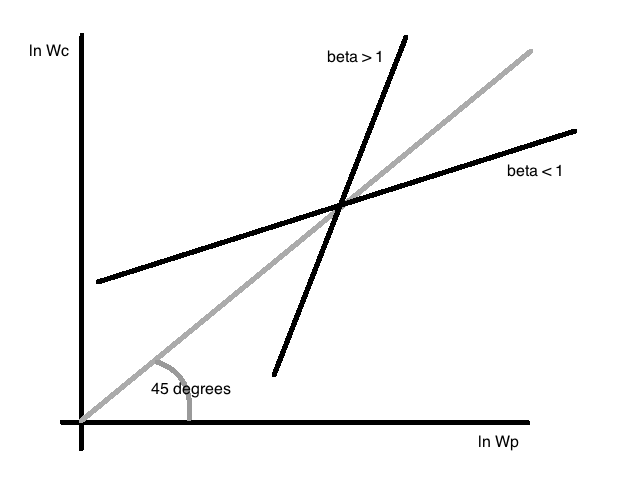
\includegraphics[width=4in, height=3in]{Plots/IGE.png}
\end{figure}
\end{center}

\indent Consider a special case where $H_{c} = R I_{c}$ with $K \geq 0$. The rate of return to investment, in this case, is $R_{y} = rK$. This means the markets are working perfectly in the sense that the returns to investment in the child are constant across different levels of parental income, $W_{p}$. Put differently, $rK$ is a constant. On the contrary, if $f_{ii} < 0$, then $R_{y} = r f_{y}$ and $R_{y}$ is strictly diminishing --$\frac{d R_{y}}{ d y} = r f_{ii}$. This implies a price effect: investment reduces the cost of investment. Given increases in $W_{p}$ increase investment, a rich parent finds it cheaper to invest. Moreover, the fact he cannot lend to a poor parent introduces an inefficiency, i.e. markets are imperfect.

\begin{center}
\begin{figure}[H] 
\caption{The Cost of Investment under Different Production Functions}
\centering
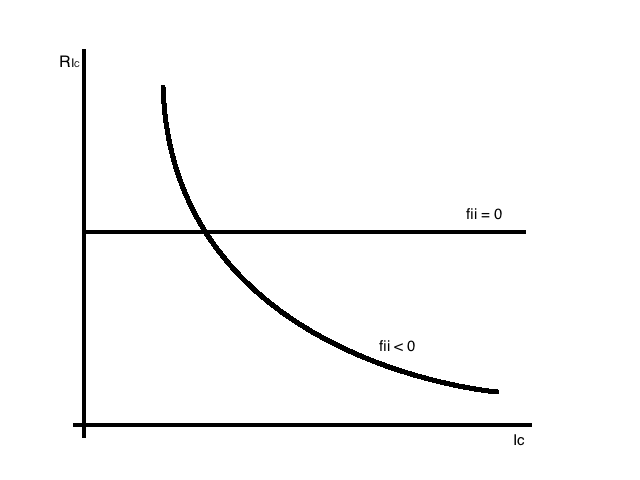
\includegraphics[width=4in, height=3in]{Plots/Rets.png}
\end{figure}
\end{center}

\indent We showed $\frac{d I_{c}}{d W_{p}} > 0$. Therefore, $\frac{d W_{c}}{d W_{p}}, \beta > 0 $. Two natural questions to ask are: (i) Is there regression to the mean? (ii) How can we study poverty? On one hand, the the empirical evidence for the US finds $\beta = .4$. This is evidence in favor of regression to the mean. On the other hand, let the variance be a measure of poverty. Hence, from \eqref{eq:ige} we know that $\var (\ln W_{c}) = \frac{\var (\epsilon_{c})}{1 - \beta^2}$ in and equilibrium where $\var (\ln W_{p})  = \var (\ln W_{c}) $. Under this assumptions, if $0 < \beta < 1$, the poverty process is well-defined and non-stationary. 

\subsection{Extending the Unisex Adult Model} \label{sec:extending}

\noindent Perhaps the most natural generalization of the unisex adult model is to allow for child's human capital to depend on parental human capital. This is, $H_{c} = f (I_{c}, H_{p})$, where $H_{p}$ denotes parental human capital. Given this is a two period model and there is only one overlapping period, $H_{p}$ is given in $t$ and we do not explicitly model how it gets there. The properties of this extended production function are the following

\begin{eqnarray}
\frac{\partial H_{c}}{\partial H_{p}} &>& 0
\frac{\partial^2 H_{c}}{\partial H_{p} \partial I_{c}} > 0. \label{eq:complements}. 
\end{eqnarray}

\indent The property in \eqref{eq:complements} is crucial as it states that that parental human capital and investment in children are complements. Importantly, the stated production function implies that the differences in production are based on the inputs and not in the technology. This is, $f(\cdot, \cdot)$ is constant across income levels, while $I_{c}, H_{p}$ may differ. This production function has a relevant consequence for economic growth. Consider the special case where $H_{c} = \psi (I_{c}) H_{p}$, where $\psi (\cdot)$ is strictly concave in its only argument. This means that the growth rate of human capital is only constant across countries if $I_{c}$ is constant since
\begin{equation}
\frac{H_{p}}{H_{c}} = \psi(I_{C}). 
\end{equation}

\noindent Given we know $I_{c}$ is a normal good under some suitable assumptions, poor economies have it difficult catching up.\\
\indent The \textit{economic problem} with this new production function is the following

\begin{equation}
\max_{I_{c}, C_{p}} \{ U_{p} (W_{p}) = U(C_{p}) + a V(W_{c}) \}
\end{equation}  

\noindent s.t.

\begin{equation}
C_{p} + I_{c} = W_{p} \label{eq:constraint1}
\end{equation}

\noindent and where $W_{c} = r f(I_{c}, H_{p})$. The first order conditions are almost the same. The equations characterizing the equilibrium in this case are functions of $H_{p}$ as well. Thus, we can use the implicit function theorem to ask what happens to the optimal decision if $C_{p}$ and $I_{c}$ as $H_{p}$ increases. To make the algebra simpler, assume $\frac{\partial W_{p}}{\partial H_{p}} = 0$ through some taxation scheme. This is \textit{with loss of generality} but it is not the focus of our discussion. Thus we have

\begin{align*}
\begin{bmatrix}
\frac{\partial C_p}{dH_p} \\
\frac{\partial I_c}{dH_p}
\end{bmatrix} &= \frac{-1}{D} \begin{bmatrix}
                                \ \ 1 & - a r (f_{II} V' + r f_I f_I V'')\ \ \\
                                \ \ -1 & -V''(C_p)\ \
                             \end{bmatrix} \cdot \begin{bmatrix}
                                                    a r [f_{IH} V'_c + f_I V'' r f_H] \\
                                                    0
                                                 \end{bmatrix} \\
              &= \begin{bmatrix}
                    \frac{\overbrace{-a r f_{IH} V'}^{ < 0} - \overbrace{a r f_y V'' r f_H}^{> 0}}{D} \\
                    \overbrace{+ (\underbrace{a r f_{IH} V'}_{>})}^{> 0} \overbrace{+ (\underbrace{a r f_I V'' r f_H}_{<})}^{< 0}
                 \end{bmatrix} \\
\end{align*}


\noindent where $D$ is defined as in  Section \ref{sec:unisex}.\\
\indent We focus on $\frac{\partial I_{c}}{\partial H_{p}}$. The income effect diminishes $H_{p}$. Greater $H_{p}$ makes the parent richer and, therefore, he consumes more for himself and invests less in the child. The substitution effect increases $H_{p}$. Given $I_{c}$ and $H_{p}$ are complements, an increase in $H_{p}$ decreases the price of $I_{c}$. Thus, it is cheaper to invest and parents do it more. In this model, it remains theoretically unclear if more educated parents, i.e. parents with greater $H_{p}$, spend more or less in their children. Put differently, this model leaves as an empirical question what are the relative magnitudes of the income and substitution effects so that the sign of $\frac{\partial I_{c}}{\partial H_{p}}$ becomes clear.\\

\subsection{Efficiency vs. Equity}

\begin{center}
\begin{figure}[H] 
\caption{Investment and its Cost without Parental Human Capital}
\label{fig:effeq}
\centering
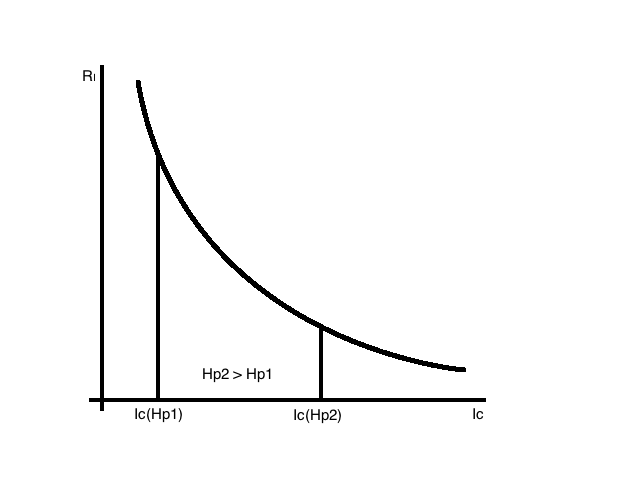
\includegraphics[width=4in, height=3in]{Plots/EffEq.png}
\end{figure}
\end{center}

\noindent When $H_{c} = f(I_{c})$ there is no trade-off between efficiency and equity. As $I_{c}$ increases, $R_{I}$ diminishes. Thus, increasing $I_{c}$, which is relatively lower for poor people given it is a normal good, is efficient and increases equity. When $H_{c} = f(I_{c}, H_{p})$ are not as nice. For any given level of $I_{c}$, $R_{i}$ is higher for a family with a parent with low human capital. Thus, it is more efficient to invest in the human capital of the child with a relatively higher human capital --which drives inequality from generation to generation. The former case is in Figure~\ref{fig:effeq} while the latter is in Figure~\ref{fig:effeff}. 

\begin{center}
\begin{figure}[H] 
\caption{Investment and its Cost with Parental Human Capital}
\label{fig:effeff}
\centering
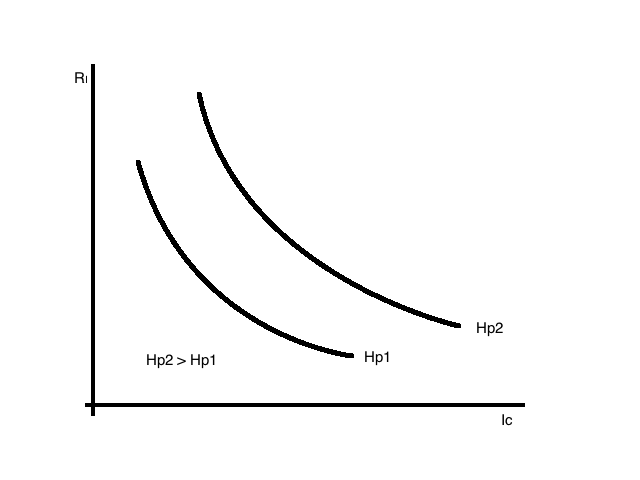
\includegraphics[width=4in, height=3in]{Plots/EffEff.png}
\end{figure}
\end{center}

\subsection{Abilities}

\noindent Bringing a single dimension of innate abilities to the model is direct. Let $A_{c}$ denote them and note we take them as given in $t$. In this extension $H_{c} = f (I_{c}, H_{p}, A_{c})$ with $\frac{\partial H_{c}}{ A_{c}} > 0$. If parental human capital and child ability are complements it is straightforward  to show that we cannot sign $\frac{\partial I_{c}}{\partial A_{c}}$ because the income and substitution effects are going in opposite directions as in Subsection~\ref{sec:extending}. Thus, it is not possible to sign the \textit{direct effect}. \\
\indent From the model, it is easy to see that $\frac{\partial W_{c}}{\partial A_{c}}$.  If it is also the case that $\frac{\partial W_{p}}{\partial A_{p}}$ due to $\frac{\partial H_{p}}{\partial A_{p}}$  , an abler parent invests more in his child through an income effect of $A_{p}$ on income, which is an \textit{indirect effect}. As in the case of parental human capital, it is more efficient to invest in a relatively abler child. Thus, efficiency and equity may go in opposite directions when ability affects human capital production. 

\end{document}